\section{Mental models and model understanding}
\subsection{Gestalt, Functionality, and fidelity}

\begin{frame}{Gestalt and Functionality}
\vspace{-2em}
\begin{columns}[T,onlytextwidth]
\column{.48\textwidth}
\begin{mynote}[Gestalt]
Forms, spatial arrangements, and structures in a learner's mental representation.
\end{mynote}
\begin{center}
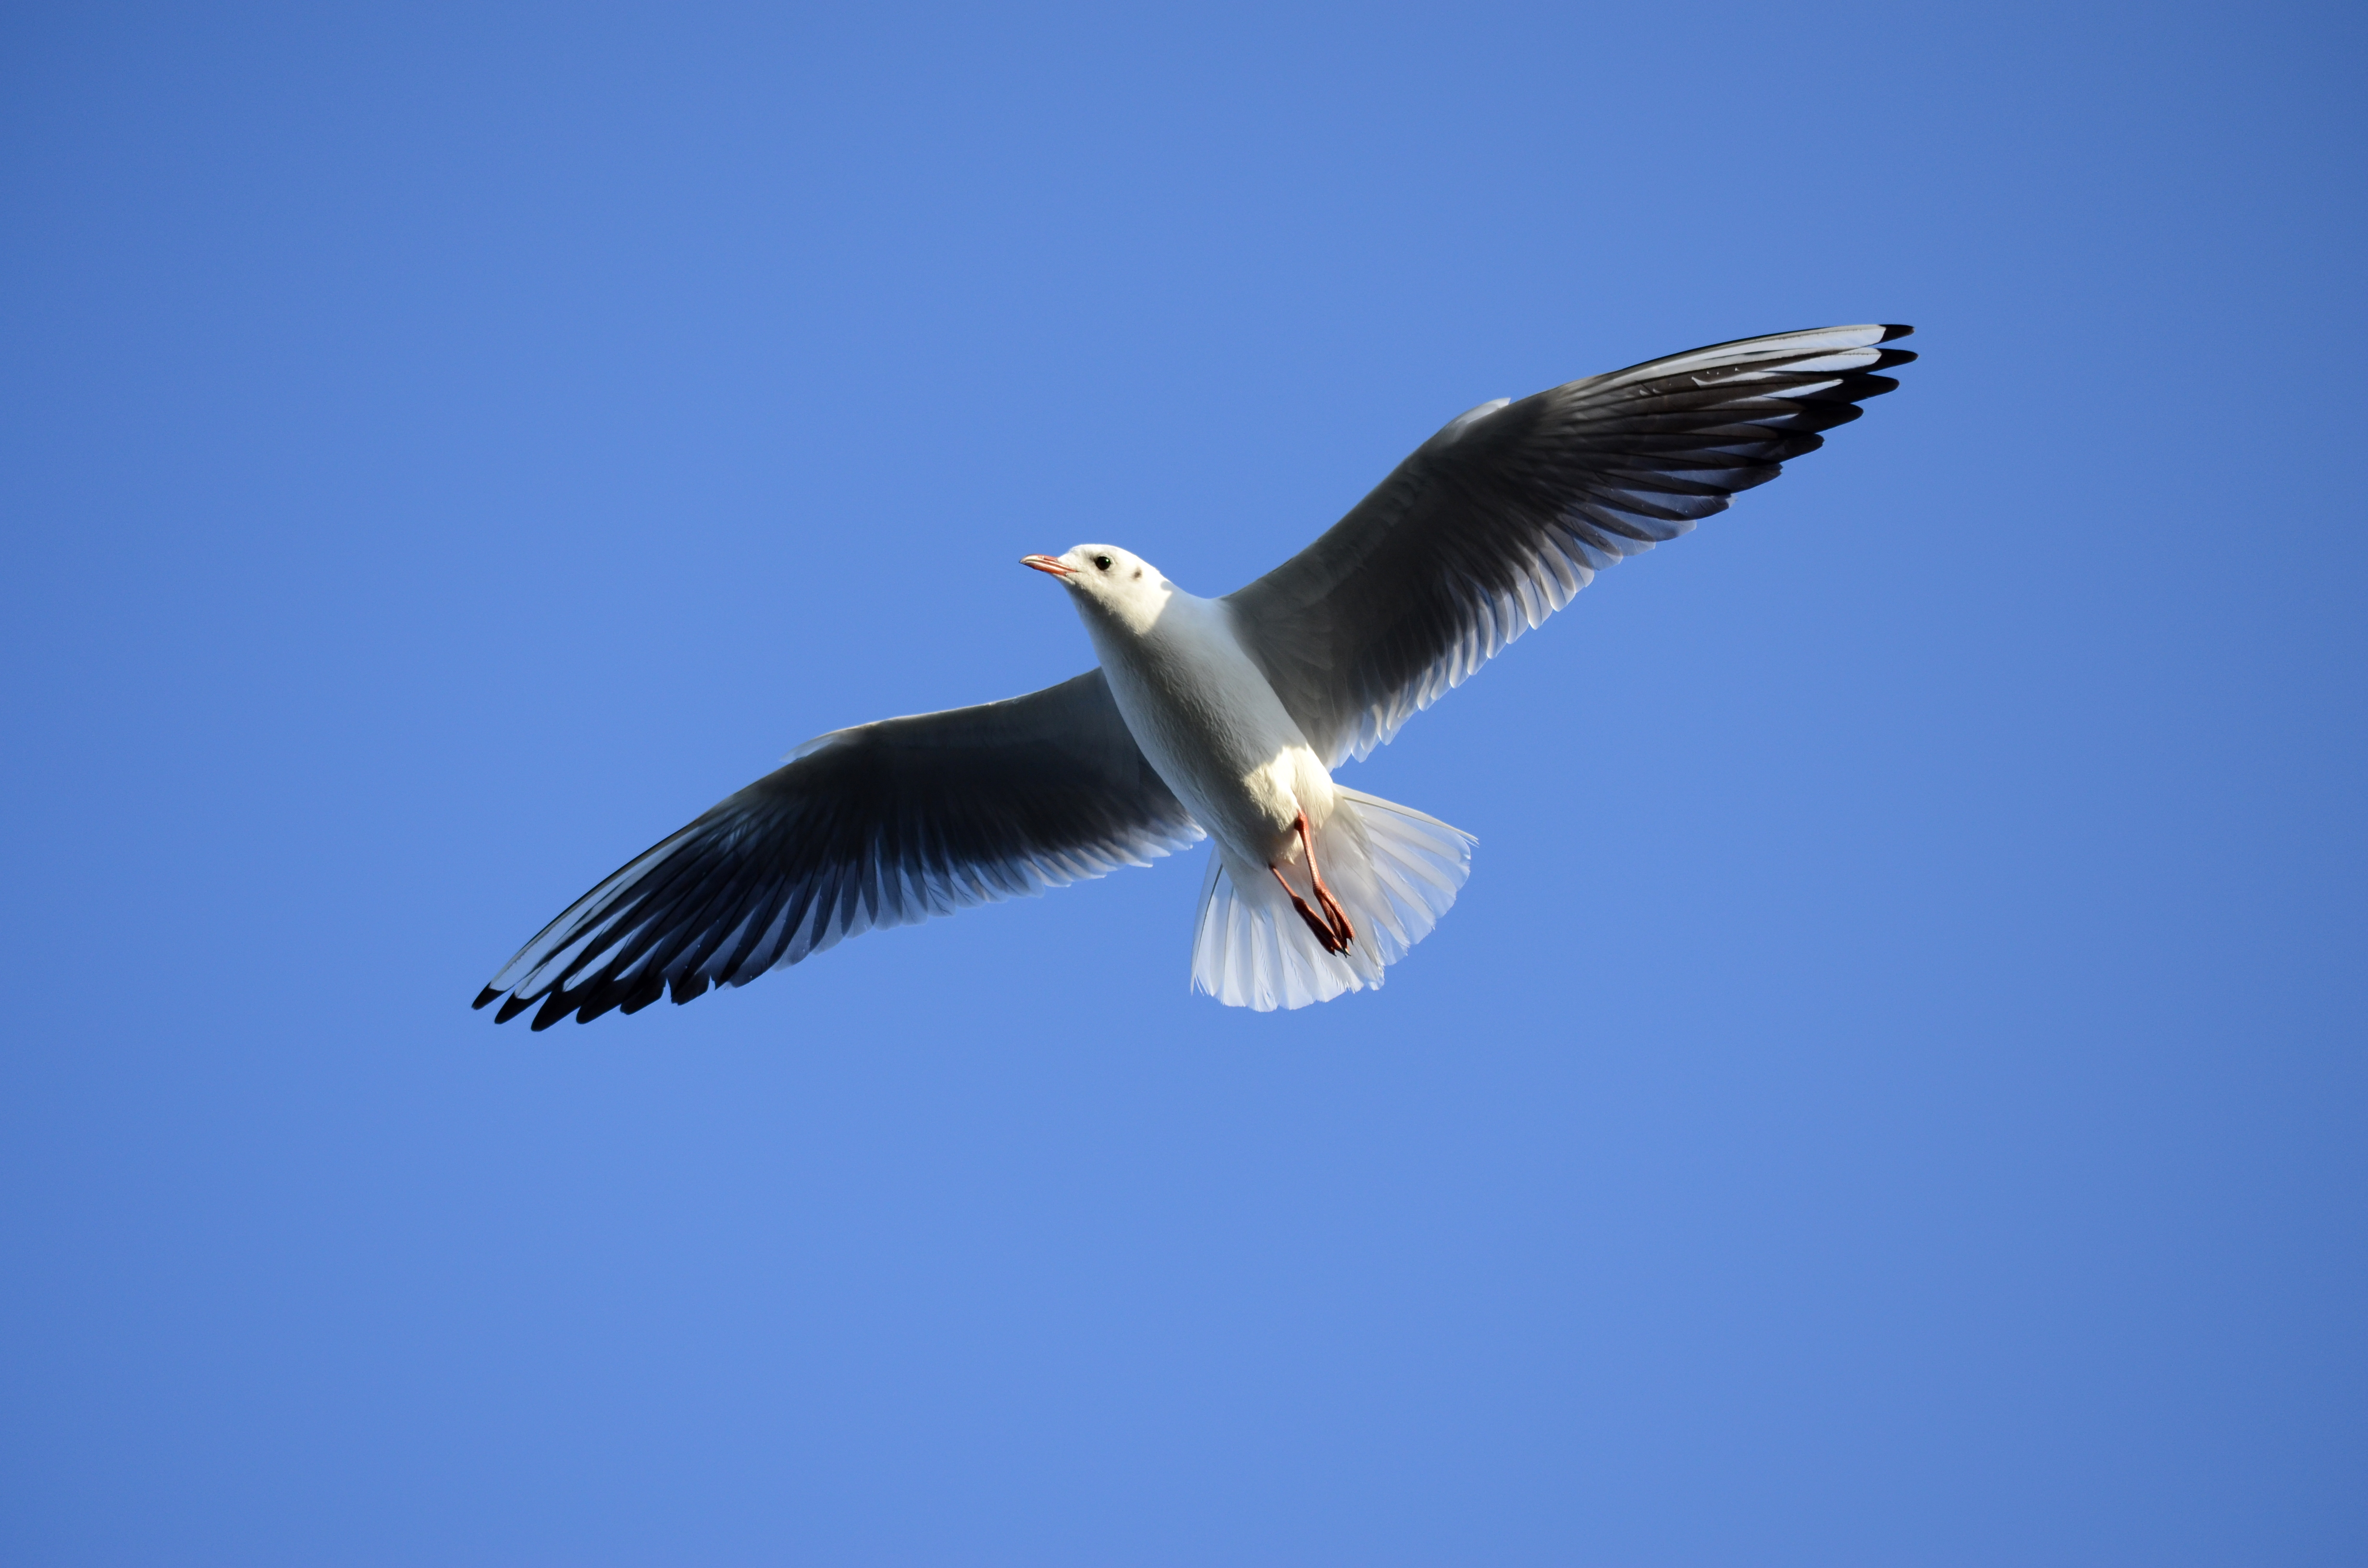
\includegraphics[width=0.7\textwidth]{images/bird.png}
\source{\citep{wiki:bird}}
\end{center}
\column{.48\textwidth}
\begin{mynote}[Functionality]
Relationships and operations used to explain behavior and make predictions.
\end{mynote}
\begin{center}
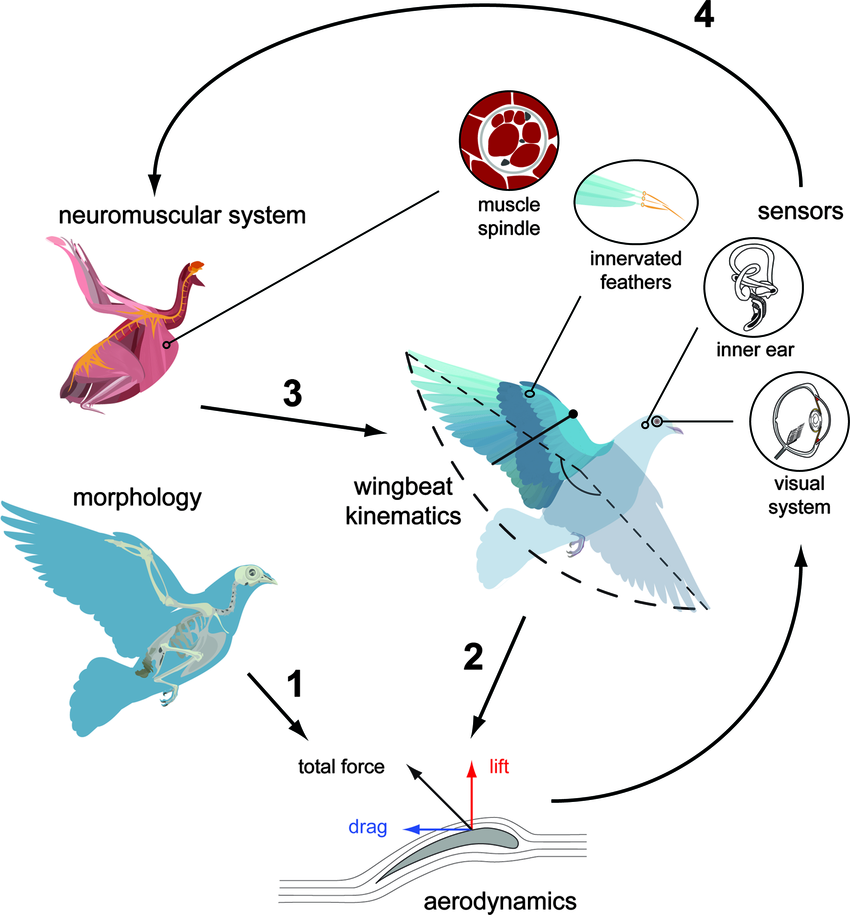
\includegraphics[width=0.5\textwidth]{images/bird_functions.png}
\source{\citep{bird_functions}}
\end{center}
\end{columns}
\slidesource{\citep{ubben2022}}
\note{Use the paired images to distinguish the forms a learner imagines from the functions encoded by those forms. The images need not contrast a realistic and an unrealistic object.}
\end{frame}

\begin{frame}{Mental models, scientific models, and the world}
\centering
\competenciesfalse\resizebox{.94\textwidth}{!}{% Adapted from the supplied figure; coordinates compressed vertically for slides.
\begin{tikzpicture}[x=.01cm,y=-.007cm]
\draw[original] (85,686) .. controls (60,660) and (46,626) .. (46,591)
.. controls (46,504) and (122,433) .. (216,433)
.. controls (310,433) and (385,504) .. (385,591)
.. controls (385,626) and (374,659) .. (350,686)
.. controls (373,714) and (385,749) .. (385,785)
.. controls (385,872) and (310,942) .. (216,942)
.. controls (122,942) and (46,872) .. (46,785)
.. controls (46,748) and (60,713) .. (85,686);
\draw[original,densely dotted] (85,686)--(350,686);
\draw[original] (650,316) .. controls (637,295) and (630,272) .. (630,248)
.. controls (630,161) and (706,90) .. (800,90)
.. controls (894,90) and (970,161) .. (970,248)
.. controls (970,273) and (964,296) .. (952,316)
.. controls (963,338) and (969,360) .. (969,384)
.. controls (969,471) and (893,541) .. (800,541)
.. controls (706,541) and (629,471) .. (629,384)
.. controls (629,359) and (637,335) .. (650,316);
\draw[original,densely dotted] (650,316)--(952,316);
\draw[original] (1180,432) rectangle (1518,942);
\draw[original] (1180,686)--(1518,686);
\draw[relation] (412,569)--(1141,569);
\draw[relation] (412,808)--(1141,808);
\draw[relation,alignmentblue] (385,571)--(632,246);
\draw[relation,alignmentblue] (385,786)--(637,466);
\draw[relation,modellingorange] (970,246)--(1180,578);
\draw[relation,modellingorange] (950,470)--(1180,812);
\node[maintext] at (216,387) {Mental models};
\node[maintext] at (797,45) {Physics model};
\node[maintext] at (1348,387) {Worldly entity};
\node[maintext] at (217,561) {Gestalt};
\node[maintext] at (217,815) {Functionality};
\node[maintext] at (800,204) {Selected forms\\and structures};
\node[maintext] at (800,402) {Selected\\functions};
\node[maintext] at (1348,561) {Sensory\\patterns};
\node[maintext] at (1348,815) {Functions};
\node[labelbox,text=alignmentblue] at (492,390) {Structural\\alignment};
\node[labelbox,text=alignmentblue] at (504,694) {Functional\\alignment};
\node[labelbox,text=modellingorange] at (1075,340) {Structural\\modelling};
\node[labelbox,text=modellingorange] at (1075,694) {Functional\\modelling};
\node[labelbox] at (777,620) {Fidelity of Gestalt};
\node[labelbox] at (792,862) {Functional fidelity};
\ifcompetencies
\node[badge] at (602,370) {1};
\node[badge] at (620,690) {2};
\node[badge] at (1160,240) {3};
\node[badge] at (1165,630) {4};
\node[badge] at (980,45) {5};
\node[badge] at (967,620) {6};
\node[badge] at (983,862) {6};
\draw[feedback] (1350,950) .. controls (1350,1006) and (1310,1020) .. (1230,1020)
-- (80,1020) .. controls (-62,1020) and (-65,956) .. (-65,861)
-- (-65,648) .. controls (-65,590) and (-28,590) .. (44,590);
\draw[feedback] (-65,850) .. controls (-65,793) and (-20,793) .. (43,793);
\node[labelbox,text=competencygreen] at (770,1020)
{\textbf{Test, evaluate, and revise}\\Update Gestalt and Functionality in response to evidence};
\node[badge] at (210,1020) {7};
\fi
\end{tikzpicture}
}
\source{Collaborative work by Judith Schmid, Malte Ubben, Fabian Hennig, Jonas Bley, and Philipp Bitzenbauer (unpublished, 2026). Black: fidelity; blue: expert alignment; orange: scientific modelling.}
\end{frame}

%\begin{frame}{Fidelity beliefs within model understanding}
%\begin{tabularx}{\textwidth}{@{}P{.23\textwidth}YY@{}}
%\toprule
%& \textbf{Fidelity of Gestalt (FG)} & \textbf{Functional Fidelity (FF)}\\
%\midrule
%Learner's belief & How closely does my model depict what the phenomenon looks like? & How adequately does my model describe how the phenomenon works?\\
%High expression & Strong belief in sensory or visual faithfulness. & Strong belief in functional adequacy.\\
%Interpretation & May encourage literal readings of abstract images. & Can support valuing prediction and explanation.\\
%\bottomrule
%\end{tabularx}\par
%\keyidea{FF and FG capture fidelity beliefs. FA and GA capture expert alignment within model understanding.}
%\source{\citep{ubben2022}; examples and application to polarization adapted for this study.}
%\end{frame}

\begin{frame}{Four aspects of model understanding}
\centering
\begin{tikzpicture}
\draw[-{Stealth},thick] (0,0)--(10.8,0) node[right] {FF};
\draw[-{Stealth},thick] (0,0)--(0,4.6) node[above] {FG};
\draw[gray,dashed] (5.2,0)--(5.2,4.2);
\draw[gray,dashed] (0,2.1)--(10.4,2.1);
\node[align=center,text width=4.7cm] at (2.6,3.2) {\textbf{Architectural}\\High FG, low FF\\Emphasis on appearance};
\node[align=center,text width=4.7cm] at (7.8,3.2) {\textbf{Dual}\\High FG, high FF\\Visual realism and function};
\node[align=center,text width=4.7cm] at (2.6,1) {\textbf{Non-developed}\\Low FG, low FF};
\node[align=center,text width=4.7cm,text=competencygreen] at (7.8,1) {\textbf{Functional}\\Low FG, high FF\\Function without literal-copy belief};
\end{tikzpicture}
\source{\citep{ubben2022}.}
\end{frame}

\subsection{Expert alignment}
\begin{frame}{Fidelity and alignment answer different questions}
\begin{columns}[T,onlytextwidth]
\column{.47\textwidth}
\textbf{Fidelity: the learner's stance}
\begin{itemize}
\item What does the learner believe the model is faithful to?
\item FG: appearance; FF: function.
\end{itemize}
\column{.49\textwidth}
\textbf{Alignment: expert correspondence}
\begin{itemize}
\item \textbf{Structural alignment (StA):} correspondence with expert-selected forms and structures.
\item \textbf{Functional alignment (FA):} correspondence with expert-selected functions.
\end{itemize}
\end{columns}
\vspace{3mm}
% A learner can reproduce the correct sphere diagram while believing it is a physical sphere surrounding the light beam.
\keyidea{High structural alignment can coexist with high FG.}
% \source{Terminology from the supplied synthesis. Structural alignment is denoted GA (Gestalt alignment) in this study.}
\end{frame}

\begin{frame}{Visualization and the multimedia effect}
\small
\vspace{-0.3em}
\begin{myalert}[Multimedia principle]
Combining words with relevant pictures can benefit learners more than words alone.
\source{\citep{Mayer2005Cognitive}}
% Learners need to connect the verbal and pictorial representations with their prior knowledge.
\end{myalert}

\begin{mynote}[DeFT: Design, Functions, Tasks]
\begin{itemize}
    \item \textbf{Design:} The number of representations,
    how information is distributed, the form, the order, and how the translations are highlighted.
    \item \textbf{Functions:} Representations can
    \textbf{complement} each other,
    \textbf{constrain} interpretations, and support the
    construction of \textbf{deeper understanding}.
    \item \textbf{Tasks:} The cognitive tasks required for learning with multiple representations: understanding the representations, their relationships, and selecting accordingly.
\end{itemize}
\vspace{-0.3em}
\source{\citep{ainsworth2006}}
\end{mynote}
%\vspace{-0.3em}
% \keyidea{The sphere may support functional reasoning,
% but connecting it with the other views also creates
% cognitive demands.}

\note{
The multimedia principle motivates combining verbal and
pictorial information. It does not imply that adding more
visualizations necessarily improves learning.

Both study conditions already contain multiple representations.
Our comparison therefore examines the contribution of an
additional representation, rather than directly testing
words plus pictures against words alone.

Applied to this study, the sphere may complement Jones notation
and the spatial wave graph by making state relationships and
transformations visible. Correspondences between the views may
constrain misleading interpretations. Connecting their shared
functional relationships may support deeper understanding.

These are proposed functions, not guaranteed effects.
Learners must understand the sphere's conventions and connect
them to the other representations. These demands may also
produce difficulty or additional cognitive load.

In DeFT, ``Tasks'' refers to the cognitive work required of
learners. It does not imply additional interview activities.
Think-aloud observations capture spontaneous reasoning during
the existing applet tasks, without added questions or prompts.
}
\end{frame}

\begin{frame}{Two pathways for an additional visualization}
\begin{columns}[T,onlytextwidth]
\column{.48\textwidth}
\begin{mynote}[Representational support]
\begin{itemize}
\item Complement by allowing different strategies to solve problems.
\item Connect notation, geometry, and optical transformations.
\item Support expert-aligned explanations and predictions.
\end{itemize}
\end{mynote}
\column{.48\textwidth}
\begin{mynote}[Spontaneous reflection]
\begin{itemize}
\item Encounter different representations of the same state.
\item Reconsider literal interpretations.
\item Attend to shared functions and limits.
\end{itemize}
\end{mynote}
\end{columns}
\keyidea{Due to the multimedia principle, expert alignment may improve even when fidelities remain stable. %Both contribute to model understanding.
}
% \source{Multiple representations: \citep{ainsworth2006}.}
\note{Visualization does not guarantee expert alignment. Prior knowledge and the demands of translating between representations may affect learning. Reflection, if expressed, arises during existing applet tasks. We do not add reflection prompts or follow-up questions.}
\end{frame}
